\documentclass[12pt]{article}
\usepackage{amsmath}
\usepackage{amssymb}
\usepackage[letterpaper,margin=0.85in,centering]{geometry}
\usepackage{fancyhdr}
\usepackage{enumerate}
\usepackage{lastpage}
\usepackage{multicol}
\usepackage{graphicx}

\reversemarginpar

\pagestyle{fancy}
\cfoot{}
\lhead{Math 1560}\chead{Test \# 4 Solutions}\rhead{June 8th, 2017}
%\rfoot{Total: 10 points}
%\chead{{\bf Name:}}
\newcommand{\points}[1]{\marginpar{\hspace{24pt}[#1]}}
\newcommand{\skipline}{\vspace{12pt}}
%\renewcommand{\headrulewidth}{0in}
\headheight 30pt

\newcommand{\di}{\displaystyle}
\newcommand{\abs}[1]{\lvert #1\rvert}
\newcommand{\len}[1]{\lVert #1\rVert}
\renewcommand{\i}{\mathbf{i}}
\renewcommand{\j}{\mathbf{j}}
\renewcommand{\k}{\mathbf{k}}
\newcommand{\R}{\mathbb{R}}
\newcommand{\aaa}{\mathbf{a}}
\newcommand{\bbb}{\mathbf{b}}
\newcommand{\ccc}{\mathbf{c}}
\newcommand{\dotp}{\boldsymbol{\cdot}}
\newcommand{\bbm}{\begin{bmatrix}}
\newcommand{\ebm}{\end{bmatrix}}                   
                  
\begin{document}


%\author{Instructor: Sean Fitzpatrick}
\thispagestyle{fancy}
%\noindent{{\bf Name and student number:}}

 \begin{enumerate}
 \item  Find the absolute maximum and minimum of $f(x)=x+\dfrac{4}{x}$ on $[1,4]$. \points{4}

\medskip

 We first check that the end point values are given by $f(1) = 1+4/1 =5$ and $f(4) = 4+4/4=5$.

 The derivative of $f$ is given by
\[
 f'(x) = 1-\frac{4}{x^2} = \frac{x^2-4}{x^2} = \frac{(x-2)(x+2)}{x^2},
\]
 so $f'(x)=0$ for $x=2$ and $x=-2$. Of these values, only $2$ is in the interval $[1,4]$, so we check the critical value $f(2) = 2+4/2 = 4$.

 Comparing values, we see that the absolute maximum value is given by $5=f(1)=f(4)$, and the absolute minimum value is $4=f(2)$.

 \bigskip

 \item A 5 metre long ladder is leaning against a vertical wall. If the base of the ladder is being pulled away from the wall at a rate of $1/3$ m/s, how fast is the top of the ladder sliding down the wall when it is 3 m from the ground? \points{4}\\
 
 \begin{multicols}{2}
  \begin{center}
   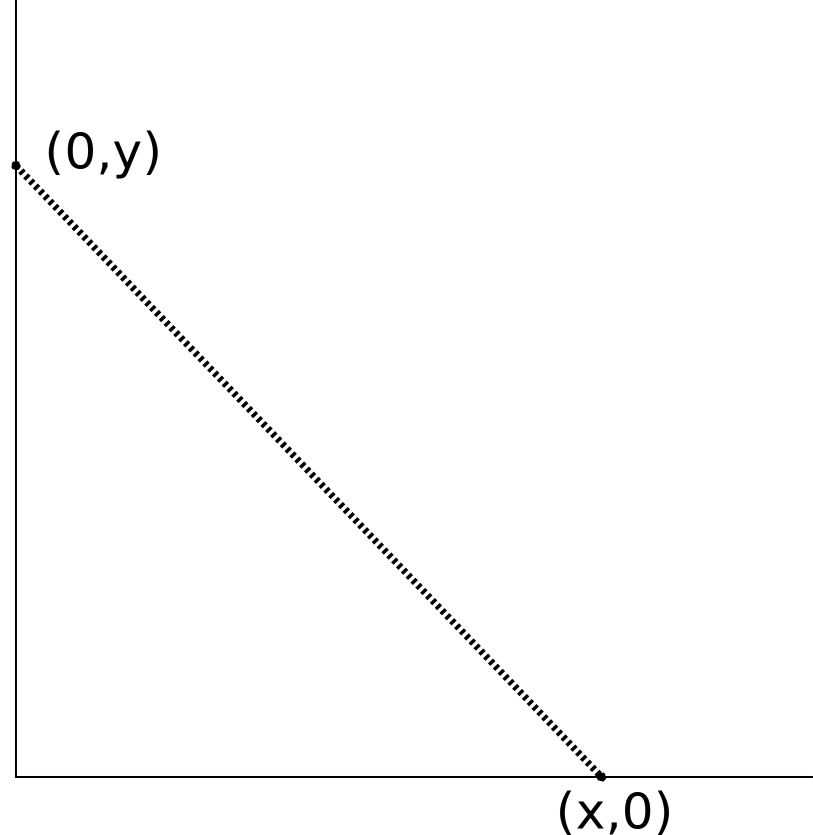
\includegraphics[width=0.8\columnwidth]{T4-2sol}
  \end{center}
  \columnbreak
  Referring to the diagram on the left, since our ladder has a length of 5, we must have 
\[
 x^2+y^2=5^2.
\]
 Since the ladder is being pulled away from the wall, $x$ is increasing, so $\frac{dx}{dt}=\frac{1}{3}$. Differentiating both sides of the above equation with respect to $t$, we find that
\[
 2x\frac{dx}{dt}+2y\frac{dy}{dt}=0.
\]
 \end{multicols}
When the top of the ladder is 3 m from the ground, we have $y=3$, and thus $x^2+3^2=5^2$, giving us $x=4$. Solving for $\dfrac{dy}{dt}$, we find
\[
 \frac{dy}{dt} = -\frac{x}{y}\frac{dx}{dt} = -\frac{4}{3}\left(\frac{1}{3}\right) = -\frac{4}{9},
\]
so the ladder is sliding down the wall at a rate of $4/9$ m/s.
 

\newpage

 \item Find the area of the largest rectangle that can be inscribed in a \textit{semicircle} of radius $R$, if one side of the rectangle must lie along the diameter of the semicircle. \points{4}

\bigskip

 \begin{multicols}{2}
  \begin{center}
   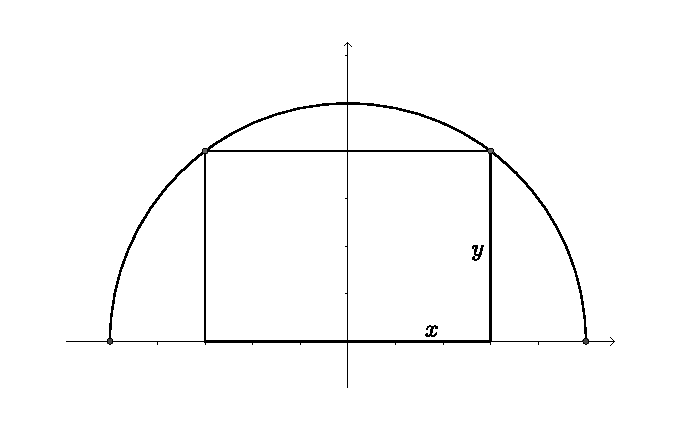
\includegraphics[width=0.9\columnwidth]{TT4-3sol}
  \end{center}
\columnbreak
 We draw our rectangle as shown on the left. Note that if the rectangle is not symmetric about the $y$-axis, then we can increase the area by lengthening one side of the base, so our rectangle is as shown, with height $y$ and base length $2x$. Since $(x,y)$ is a point on the circle, we have $x^2+y^2=R^2$. Solving for $y$ gives us $y=\sqrt{R^2-x^2}$.
 \end{multicols}
The area of our rectangle is thus given by $A(x) = 2x\sqrt{R^2-x^2}$, with $0\leq x\leq R$. We note that $A(0)=A(R)=0$, so the maximum must occur at a critical point. We have
\begin{align*}
 A'(x) & = 2\sqrt{R^2-x^2}+2x\left(\frac{-x}{\sqrt{R^2-x^2}}\right)\\
& = \frac{2(R^2-x^2)-2x^2}{\sqrt{R^2-x^2}} = \frac{2R^2-4x^2}{\sqrt{R^2-x^2}}.
\end{align*}
It follows that $A'(x)=0$ for $2R^2-4x^2=0$, giving us $x^2=\dfrac{R^2}{2}$, so $x=\dfrac{R}{\sqrt{2}}$ (positive root since $x>0$). For this value of $x$, we have
\[
 y = \sqrt{R^2-R^2/2} = \sqrt{R^2/2} = \frac{R}{\sqrt{2}}.
\]
The area of our rectangle is therefore
\[
 A = 2\left(\frac{R}{\sqrt{2}}\right)^2 = R^2.
\]

\medskip

 \item Use a linear approximation to estimate the value of $\sqrt{9.2}$. \points{4}

\medskip

 We use $f(x)=\sqrt{x}$ as our function, and approximate near $a=9$. We have
\[
 l(x) = f(9)+f'(9)(x-9) = \sqrt{9}+\frac{1}{2\sqrt{9}}(x-9) = 3+\frac{1}{6}(x-9).
\]
Thus, our approximation is
\[
 \sqrt{9.2} \approx l(9.2) = 3+\frac{1}{6}(9.2-9) = 3+\frac{1}{6}(0.2) = 3.0333.
\]
(This is a pretty good estimate compared to the calculator value of $3.03315$.

\end{enumerate}





\end{document}